
\graphicspath{{figures/trig/}}
\chapter{Trigonometry}\label{app trig}


\section{Trigonometry --- Graphs}\label{app sec trig graphs}
\begin{center}
\begin{tabular}{ccc}
$\sin \theta$ & $\cos \theta$ & $\tan \theta$
\\
\begin{tikzpicture} 
\begin{axis}[
  axis x line=center, axis y line=center, 
  ymax=1.1,ymin=-1.1, ytick={-1,1},
  xtick={-3.141592654,-1.570796327,1.570796327,3.141592654,4.71238898,6.283185307},
  xticklabels={$-\pi$, $-\frac{\pi}{2}$, $\frac{\pi}{2}$, $\pi$, $\frac{3\pi}{2}$,$2\pi$}
  ]
\addplot[blue,domain=-1.1*pi:2.1*pi,samples=100] {sin(deg(x))}; 
\end{axis}
\end{tikzpicture}
&
\begin{tikzpicture} 
\begin{axis}[
  axis x line=center, axis y line=center, 
  ymax=1.1,ymin=-1.1, ytick={-1,1},
  xtick={-3.141592654,-1.570796327,1.570796327,3.141592654,4.71238898,6.283185307},
  xticklabels={$-\pi$, $-\frac{\pi}{2}$, $\frac{\pi}{2}$, $\pi$, $\frac{3\pi}{2}$,$2\pi$}
  ]
\addplot[blue,domain=-1.1*pi:2.1*pi,samples=100] {cos(deg(x))}; 
\end{axis}
\end{tikzpicture}
&
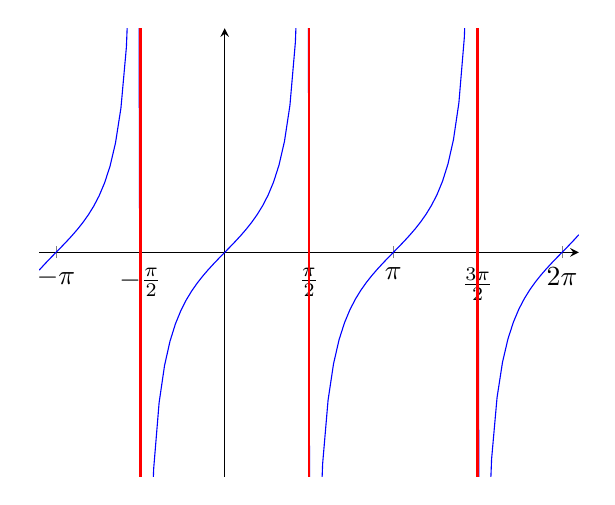
\begin{tikzpicture} 
\begin{axis}[
  axis x line=center, axis y line=center, 
  ymax=4.1,ymin=-4.1, ymajorticks=false,
  xtick={-3.141592654,-1.570796327,1.570796327,3.141592654,4.71238898,6.283185307},
  xticklabels={$-\pi$, $-\frac{\pi}{2}$, $\frac{\pi}{2}$, $\pi$, $\frac{3\pi}{2}$,$2\pi$}
  ]
\addplot[blue,domain=-1.1*pi:2.1*pi,samples=100] {tan(deg(x))}; 

\addplot[line width=1pt,red] coordinates {(-1.570796327,4.15) (-1.570796327,-4.15)};
\addplot[line width=1pt,red] coordinates {(1.570796327,4.15) (1.570796327,-4.15)};
\addplot[line width=1pt,red] coordinates {(4.71238898,4.15) (4.71238898,-4.15)};
\end{axis}
\end{tikzpicture}
\end{tabular}
\end{center}

\section{Trigonometry --- Special Triangles}
\begin{center}
  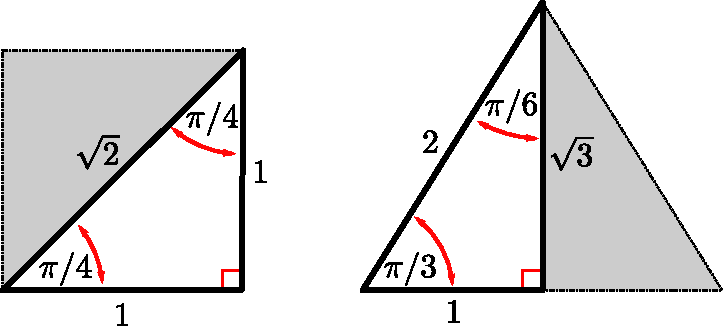
\includegraphics[height=4cm]{special_triangles}
\end{center}
From the above pair of special triangles we have
\begin{align*}
  \sin \frac{\pi}{4} &= \frac{1}{\sqrt{2}} &  \sin \frac{\pi}{6} &= \frac{1}{2} & \sin \frac{\pi}{3} &= \frac{\sqrt{3}}{2} \\   
  \cos \frac{\pi}{4} &= \frac{1}{\sqrt{2}} &  \cos \frac{\pi}{6} &= \frac{\sqrt{3}}{2} & \cos \frac{\pi}{3} &= \frac{1}{2} \\   
  \tan \frac{\pi}{4} &= 1 &  \tan \frac{\pi}{6} &= \frac{1}{\sqrt{3}} & \tan 
\frac{\pi}{3} &= \sqrt{3}
\end{align*}

\section{Trigonometry --- Simple Identities}
\begin{itemize}
 \item Periodicity
\begin{align*}
  \sin(\theta+2\pi) &= \sin(\theta) &
  \cos(\theta+2\pi) &= \cos(\theta) 
\end{align*}
\item Reflection
\begin{align*}
  \sin(-\theta)&=-\sin(\theta) & \cos(-\theta) &=\cos(\theta) 
\end{align*}
\item Reflection around $\pi/4$
\begin{align*}
\sin\left(\tfrac{\pi}{2}-\theta\right)&=\cos\theta &
\cos\left(\tfrac{\pi}{2}-\theta\right)&=\sin\theta 
\end{align*}
\item Reflection around $\pi/2$
\begin{align*}
\sin\left(\pi-\theta\right)&=\sin\theta &
\cos\left(\pi-\theta\right)&=-\cos\theta 
\end{align*}
\item Rotation by $\pi$
\begin{align*}
\sin\left(\theta+\pi\right)&=-\sin\theta &
\cos\left(\theta+\pi\right)&=-\cos\theta 
\end{align*}
\item Pythagoras
\begin{align*}
\sin^2\theta + \cos^2 \theta &=1  \\
\tan^2\theta + 1  &= \sec^2\theta \\
1 + \cot^2 \theta &=\csc^2\theta
\end{align*}
\item $\sin$ and $\cos$ building blocks
\begin{align*}
\tan\theta=\frac{\sin\theta}{\cos\theta}\qquad
\csc\theta=\frac{1}{\sin\theta}\qquad
\sec\theta=\frac{1}{\cos\theta}\qquad
\cot\theta=\frac{\cos\theta}{\sin\theta}=\frac{1}{\tan\theta}
\end{align*}
\end{itemize}

\section{Trigonometry --- Add and Subtract Angles}\label{sec trig add}
\begin{itemize}
 \item Sine
\begin{align*}
  \sin(\alpha \pm \beta) &= \sin(\alpha)\cos(\beta) \pm \cos(\alpha)\sin(\beta)
  \end{align*}
 \item Cosine
\begin{align*}
  \cos(\alpha \pm \beta) &= \cos(\alpha)\cos(\beta) \mp \sin(\alpha)\sin(\beta)
\end{align*}
\item Tangent
\begin{align*}
\tan(\alpha+\beta)&=\frac{\tan\alpha+\tan\beta}{1-\tan\alpha\tan\beta} \\
\tan(\alpha-\beta)&=\frac{\tan\alpha-\tan\beta}{1+\tan\alpha\tan\beta}
\end{align*}
\item Double angle
\begin{align*}
  \sin(2\theta) &= 2\sin(\theta)\cos(\theta) \\
  \cos(2\theta) &= \cos^2(\theta) - \sin^2(\theta) \\
  &= 2\cos^2(\theta) - 1   \\
  &= 1 - 2\sin^2(\theta) \\
  \tan(2\theta) &= \frac{2\tan(\theta)}{1-\tan^2\theta} \\
\cos^2\theta&=\frac{1+\cos(2\theta)}{2} \\
\sin^2\theta&=\frac{1-\cos(2\theta)}{2} \\
\tan^2\theta&=\frac{1-\cos(2\theta)}{1+\cos(2\theta)}
\end{align*}
\item Products to sums
\begin{align*}
\sin(\alpha)\cos(\beta)&= \frac{\sin(\alpha+\beta) +  \sin(\alpha-\beta)}{2} \\
\sin(\alpha)\sin(\beta)&= \frac{\cos(\alpha-\beta) - \cos(\alpha+\beta)}{2}\\
\cos(\alpha)\cos(\beta)&= \frac{\cos(\alpha-\beta) + \cos(\alpha+\beta)}{2}
\end{align*}
\item Sums to products
\begin{align*}
\sin\alpha+\sin\beta 
           &= 2 \sin\frac{\alpha+\beta}{2}\cos\frac{\alpha-\beta}{2} \\
\sin\alpha-\sin\beta 
           &= 2 \cos\frac{\alpha+\beta}{2}\sin\frac{\alpha-\beta}{2} \\
\cos\alpha+\cos\beta  
           &= 2 \cos\frac{\alpha+\beta}{2}\cos\frac{\alpha-\beta}{2} \\
\cos\alpha-\cos\beta 
           &= -2 \sin\frac{\alpha+\beta}{2}\sin\frac{\alpha-\beta}{2}
\end{align*}

\end{itemize}

\section{Inverse Trigonometric Functions}\label{sec inv trig}
\begin{center}
\renewcommand{\arraystretch}{1.5}
\begin{tabular}{|c|c|c|}
\hline
$\arcsin x$ & $\arccos x$ & $\arctan x$\\
\hline
Domain: $-1 \leq x \leq 1$&
Domain: $-1 \leq x \leq 1$&
Domain: all real numbers\\
Range: $-\frac{\pi}{2} \leq \arcsin x \leq \frac{\pi}{2}$&
Range: $0 \leq \arccos x \leq \pi$&
Range: $-\frac{\pi}{2} < \arctan x < \frac{\pi}{2}$\\
\hline
\begin{tikzpicture} 
\begin{axis}[
  legend pos = north west,
  axis x line=center, axis y line=center, 
  xmax=1.1,xmin=-1.1, xtick={-1,1},
  ymin=-2, ymax=2,
  ytick={-1.570796327,1.570796327},
  yticklabels={$-\nicefrac{\pi}{2}$, $\nicefrac{\pi}{2}$}
  ]
\addplot[blue, line width=1pt, domain=-1:1,samples=100] {asin(x)/180*pi}; 
% \legend{$\arcsin \theta$}
\end{axis}
\end{tikzpicture}
&
%\raisebox{0.15in}{
\begin{tikzpicture} 
\useasboundingbox (0,0) rectangle (5,4.2);
\begin{axis}[
  axis x line=center, axis y line=center, 
  xmax=1.1,xmin=-1.1, xtick={-1,1},
  ymin=-0.3,ymax=3.4,
  ytick={0,1.570796327,3.141592654},
  yticklabels={0,$\nicefrac{\pi}{2}$, $\pi$}
  ]
 \addplot[blue, line width=1pt, domain=-1:1,samples=100] {acos(x)/180*pi}; 
% \legend{$\cos \theta$}
\end{axis}
\end{tikzpicture}
%}
&
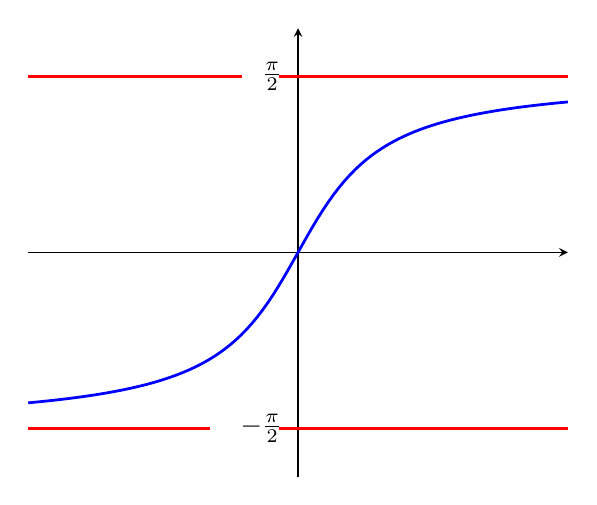
\begin{tikzpicture} 
\begin{axis}[
  legend pos = north west,
  axis x line=center, axis y line=center, 
  xmax=4.3,xmin=-4.3, xmajorticks=false,
  ymin=-2,ymax=2,
  ytick={-1.570796327,1.570796327},
  yticklabels={$-\frac{\pi}{2}$, $\frac{\pi}{2}$}
  ]
\addplot[blue, line width=1pt, domain=-4.3:4.3,samples=100] {atan(x)/180*pi}; 
% \legend{$\tan \theta$}

\addplot[line width=1pt,red] coordinates {(4.3,-1.570796327) (-0.3,-1.570796327)};
\addplot[line width=1pt,red] coordinates {(-1.4,-1.570796327) (-4.3,-1.570796327)};
\addplot[line width=1pt,red] coordinates {(4.3,1.570796327) (-0.3,1.570796327)};
\addplot[line width=1pt,red] coordinates {(-0.9,1.570796327) (-4.3,1.570796327)};
\end{axis}
\end{tikzpicture}
\\ \hline
\end{tabular}
\renewcommand{\arraystretch}{1}
\end{center}
Since these functions are inverses of each other we have
\begin{align*}
  \arcsin(\sin \theta) &= \theta & -\frac{\pi}{2} \leq \theta \leq \frac{\pi}{2} \\
  \arccos(\cos \theta) &= \theta & 0 \leq \theta \leq \pi \\
  \arctan(\tan \theta) &= \theta & -\frac{\pi}{2} \leq \theta \leq \frac{\pi}{2}	
\end{align*}
and also
\begin{align*}
  \sin(\arcsin x) &= x & -1 \leq x \leq 1 \\
  \cos(\arccos x) &= x & -1 \leq x \leq 1 \\
  \tan(\arctan x) &= x & \text{any real $x$}
\end{align*}
%The compositions of trignometric and inverse trigonometric functions are
%\begin{align*}
%  \sin( \arcsin x ) &= x & 
%  \sin( \arccos x ) &= \sqrt{1-x^2} & 
%  \sin( \arctan x ) &= \frac{x}{\sqrt{1+x^2}} \\ 
%%
%  \cos( \arcsin x ) &= \sqrt{1-x^2} & 
%  \cos( \arccos x ) &= x &
%  \cos( \arctan x ) &= \frac{1}{\sqrt{1+x^2}} \\ 
%%
%  \tan( \arcsin x ) &= \frac{x}{\sqrt{1-x^2}} & 
%  \tan( \arccos x ) &= \frac{\sqrt{1-x^2}}{x} &
%  \tan( \arctan x ) &= x 
%\end{align*}

\begin{center}
\renewcommand{\arraystretch}{1.5}
\begin{tabular}{|c|c|c|}
\hline
$\arccsc x$ & $\arcsec x$ & $\arccot x$\\
\hline
Domain: $|x|\ge 1$&
Domain: $|x|\ge 1$&
Domain: all real numbers\\
Range: $-\frac{\pi}{2} \leq \arccsc x \leq \frac{\pi}{2}$&
Range: $0 \leq \arcsec x \leq \pi$&
Range: $0 < \arccot x < \pi$\\[-0.1in]
       $\arccsc x \ne 0$ &
       $\arcsec x \ne \frac{\pi}{2}$ &
        \\
\hline
\begin{tikzpicture} 
\begin{axis}[
  legend pos = north west,
  axis x line=center, axis y line=center, 
  xmax=4.3,xmin=-4.3, xtick={-1,1},
  ymin=-2, ymax=2,
  ytick={-1.570796327,1.570796327},
  yticklabels={$-\frac{\pi}{2}\!\!\!$, $\frac{\pi}{2}$}
  ]
\addplot[blue, line width=1pt, domain=1:4.3,samples=50] {asin(1/x)/180*pi}; 
\addplot[blue, line width=1pt, domain=-4.3:-1,samples=50] {asin(1/x)/180*pi}; 
\end{axis}
\end{tikzpicture}
&
\begin{tikzpicture} 
\useasboundingbox (0,0) rectangle (5,4.2);
\begin{axis}[
  axis x line=center, axis y line=center, 
  xmax=4.3,xmin=-4.3, xtick={-1,1},
  ymin=-0.3,ymax=3.4,
  ytick={0,1.570796327,3.141592654},
  yticklabels={0,$\frac{\pi}{2}$, $\pi$}
  ]
 \addplot[blue, line width=1pt, domain=1:4.3,samples=100] {acos(1/x)/180*pi}; 
 \addplot[blue, line width=1pt, domain=-4.3:-1,samples=100] {acos(1/x)/180*pi}; 
% \legend{$\cos \theta$}
\end{axis}
\end{tikzpicture}
&
\begin{tikzpicture} 
\begin{axis}[
  legend pos = north west,
  axis x line=center, axis y line=center, 
  xmax=4.3,xmin=-4.3, xmajorticks=false,
  ymin=-0.3,ymax=3.4,
  ytick={0,1.570796327,3.141592654},
  yticklabels={0,$\frac{\pi}{2}$, $\pi$}
  ]
\addplot[blue, line width=1pt, domain=-4.3:-0.01,samples=100] {atan(1/x)/180*pi + pi}; 
\addplot[blue, line width=1pt, domain=0.01:4.3,samples=100] {atan(1/x)/180*pi}; 
% \legend{$\tan \theta$}

\addplot[line width=1pt,red] coordinates {(4.3,3.141592654) (-0.3,3.141592654)};
\addplot[line width=1pt,red] coordinates {(-0.9,3.141592654) (-4.3,3.141592654)};
\end{axis}
\end{tikzpicture}
\\ \hline
\end{tabular}
\renewcommand{\arraystretch}{1}
\end{center}
Again
\begin{align*}
  \arccsc(\csc \theta) &= \theta & -\frac{\pi}{2} \leq \theta \leq \frac{\pi}{2},\ \theta\ne 0 \\
  \arcsec(\sec \theta) &= \theta & 0 \leq \theta \leq \pi,\ \theta\ne \frac{\pi}{2} \\
  \arccot(\cot \theta) &= \theta & 0 < \theta < \pi	
\end{align*}
and 
\begin{align*}
  \csc(\arccsc x) &= x & |x|\ge 1 \\
  \sec(\arcsec x) &= x & |x|\ge 1 \\
  \cot(\arccot x) &= x & \text{any real $x$}
\end{align*}













